\documentclass[12pt,fleqn]{article}\usepackage{../common}
\begin{document}
Ders 5

Permutasyonlar

Bu derste bir anlamda lineer cebirin ruhunu gormeye baslayacagiz, sadece
vektorler degil artik vektor uzaylarina bakmaya baslayacagiz, yani daha
buyuk resme odaklanacagiz. Ayrica herhangi bir uzayin alt-uzaylarini
(subspace) inceleyecegiz. 

Permutasyonlari hatirlayalim: permutasyon matrisi $P$ bir diger matrisin
satirlarini degis-tokus etmek icin kullaniliyordu. Bu isleme ihtiyacimiz
olabilir, cunku, elimizde $Ax=b$ cozerken belki de (neredeyse) mukemmel bir
$A$ olsa da bazen mesela tek bir yerdeki sifir isi bozuyor olabilir, onu
yerinden oynatirsam, duzgun bir pivot elde edersem cozum olacaktir, iste o
zaman permutasyon kullanabilirim.

Peki $A=LU$'nun bir sistemi cozerken gerekebilecek permutasyonlar ile
alakasi nedir?

$A=LU$'nin ne oldugunu hatirlayalim, 

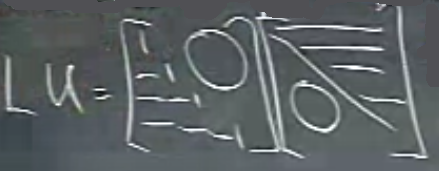
\includegraphics[height=3cm]{5_01.png}

Bu resme bakarsa, bu tur gosterilen edilmis bir $LU$ tarifini $P$'nin
olmadiginin farz ediyor, yani hic satir degis-tokusuna gerek olmadigi farz
ediliyor. Peki eger satir degis tokusu gerekseydi, bu durumu cebirsel
olarak nasil gosterirdim? 

Aslinda ustteki tanimda da $P$ ``var'', ya da oldugunu dusunebiliriz, ama
$P$ bu durumda birim matrisidir. 

Simdi bir dakika durup mesela Matlab [artik Python] lineer cebir
kutuphanelerinin cozumu nasil yaptigini dusunelim. Bu kutuphaneler pivot'in
sifir olup olmadigina bakarlar, ki herhangi bir insan da bunu yapar, ayrica
pivot'in ``yeterince buyuk olup olmadigina da'' bakilir, cunku sifira
yakin, cok kucuk pivotlar sayisal hesap baglaminda kotudur. Bu durumda
kutuphaneye ``coz'' dedigimizde kodun arka planda satir degis-tokuslari
yaptigini gorururuz, bu degisimler pur matematiksel olarak gerekli
olmayabilirler, ama hesap / sayisal acidan gereklidirler. 

Neyse, ya sayisal sebepten, ya da baska bir sebepten dolayi satir degis
tokusu gerekebilir, o zaman nihai olarak satir degisimini iceren
eliminasyon sudur:

$$ PA = LU $$

$P$ satir degis-tokusunu yapan matristir. $P$, $A$'yi ``ideal'' hale
getirir, sifirlar pivot'ta olmaz, vs. 

Bu arada bir permutasyon matrisinin yapisini hatirlayalim, temelinde bir
permutasyon matrisi satirlarinin yeri degistirilmis bir birim
matristir. Permutasyon matrisleri pek cok satir degisimi ayni anda
yapabilir, kac turlu degisim kombinasyonu vardir? 

$$ n! = n(n-1)...(3)(2)(1) $$

cunku ustteki kadar degisik satir siralamasi mumkundur, ve tum
permutasyonlari boyle hesaplayabiliriz. 

Ayrica $P$ tersi alinabilir (invertible) bir matristir, ve 

$$ P^{-1} = P^T $$

ya da 

$$ P^TP = I $$

Bu ``guzel'' bir ozellik, ve bu tur ozelliklere sahip olan matrisler bizi
ozellikle ilgilendiriyor.

Ornek

$$ 
\left[\begin{array}{rr}
1 & 3 \\
2 & 3 \\
4 & 1 
\end{array}\right]^T
 $$

Basit bir devrik islemi... Sonuc nedir?

$$ =
\left[\begin{array}{rrr}
1 & 2 & 4 \\
1 & 3 & 3 
\end{array}\right]
 $$

Devrik islemi, formulsel olarak 

$$ (A^T)_{ij} = A_{ji} $$

Simdi simetrik matrislerden bahsedelim, bunlar cok ``sevdigimiz''
matrislerden biri. Bu matrislerin guzel bir ozelligi, devrigi kendisine
esit olmasi,

$$ A^T = A $$

Mesela

$$ 
\left[\begin{array}{rrr}
3 & 1 & 7 \\
1 & 2 & 9 \\
7 & 9 & 4
\end{array}\right]
 $$

Bu tur bir matrisi ne zaman elde ederiz? Iki ustteki matris mesela $3
\times 2$ boyutunda zaten, simetrik olmasi zaten mumkun degil, cunku devrik
islemi boyut degisikligine sebep oluyor. Fakat dikdortgensel olsa bile
(cunku kare seklinde degil, yani boyutlari farkli) bir matristen acaba bir
islem uyguluyarak simetrik bir matris elde edemez miyim? Fikir: iki ustteki
matrise $R$ diyelim, $R^TR$ ile simetrik bir matris elde edebilirim. Bu
hakikaten mumkun, hatta kural olarak alabiliriz, $R^TR$ her zaman simetrik
matris verir. Ornekte gorelim, 

$$ 
\left[\begin{array}{rr}
1 & 3 \\
2 & 3 \\
4 & 1 
\end{array}\right]^T
\left[\begin{array}{rrr}
1 & 2 & 4 \\
1 & 3 & 3 
\end{array}\right]
=
\left[\begin{array}{rrr}
10 & 11 & 7 \\
11 & .. & .. \\
7 & .. & ..
\end{array}\right]
 $$  

Gerisi de ayni olacakti. Sembolik olarak gorelim, $R^TR$'in simetrik
oldugunu nasil bulurum? Onun devrigini alabilirim, ve sonucun degismemesini
kontrol edebilirim,

$$ (R^TR)^T = R^T(R^T)^T $$

$(R^T)^T$ nedir? Bir matrisin iki kere devrigini alirsam tekrar kendisine
donmus olmaz miyim? Evet. O zaman, 

$$  R^T(R^T)^T = R^T R $$

Basktaki hale donduk! Demek ki $R^TR$ bir simetrik matristir. Ispat
tamamlandi. 







\end{document}
